The model still assumes that low probability bound is 0 (i.e. that high titres correlate with immunity in a univariate model). This assumption is justified if there is a reasonable number of people in the sample who have high titres and none (or very few) of whom get infected. In the Ha Nam data (Figure \ref{HanamCounts}), there is a total of 131 observations with titres above 160. None of those subjects got infected in the corresponding season. For the Ha Nam data, the assumption of immunity at high titres is not unreasonable.

Compared to logistic regression, the scaled logit model requires a larger sample size. This is because the scaled logit model estimates an additional parameter. Hence for the same samplt size, estimates from the sclaed logit model will have larger standard errors.

Figures \ref{SclrSE}, \ref{SclrConv} and \ref{SclrMean} summarise 10,000 simulation results from the model

\begin{align*}
	\begin{gathered}
		\frac{0.5}{\text{exp}(-5 + 1.5 X)} \\
		X \sim N(2, 2^2)
	\end{gathered}
\end{align*}

Figure \ref{SclrSE} shows that standard errors of the regression estimates were consistently higher with the scaled logit model.

Figure \ref{SclrConv} shows that in order to reliably converge (under the chosen true parameter values) the scaled logit model required the sample size to be over 500. The standard logistic model always converged.

The bias of the scaled logit estimates evident in Figure \ref{SclrMean} is likely due to the fact that the subset of the simulated datasets for which the scaled logit model converged is not a random subset. Datasets for which the scaled logit model is more likely to converge have certain properties, e.g. a large number of infections, a large number of subjects with detectable titres. Label these as "informative" datasets. Informative datasets are balanced out by simulated datasets where the opposite properies occur --- small infection numbers, small numbers with detectable titres. Label these "non-informative" datasets. With a large enough sample size, we can obtain estimates from both the informative and the non-informative datasets. With a small sample size, we can obtain estimates only from the informative datasets (the model does not converge for the non-informative), i.e. a non-random subset of simulated data. Aggregating estimates only over the informative datasets leads to bias.

\begin{figure}[htp]
	\centering
	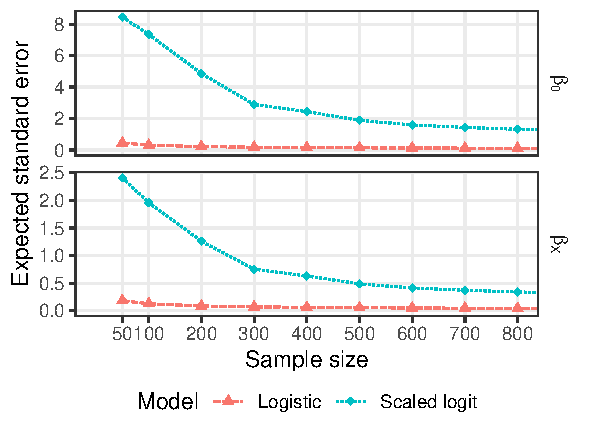
\includegraphics[width=0.69\textwidth]{../logistic-plot/vary_nsam_se.pdf}
	\caption{
		Simulation results of fitting the standard logistic and the scaled logit models to the same simulated datasets. 10,000 datasets were simulated. Shown is the mean standard error of the regression estimates from the standard logistic (the dashed line) and the scaled logit (the dotted line). Points indicate parameter values at which the simulations were performed.
	}
	\label{SclrSE}
\end{figure}

\begin{figure}[htp]
	\centering
	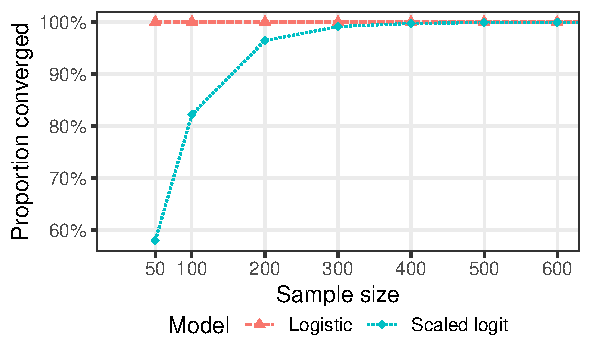
\includegraphics[width=0.69\textwidth]{../logistic-plot/vary_nsam.pdf}
	\caption{
		Simulation results of fitting the standard logistic and the scaled logit models to the same simulated datasets. 10,000 datasets were simulated. Shown is the proportion of successful attempts to fit the standard logistic (the dashed line) and the scaled logit (the dotted line) model. Points indicate parameter values at which the simulations were performed.
	}
	\label{SclrConv}
\end{figure}

\begin{figure}[htp]
	\centering
	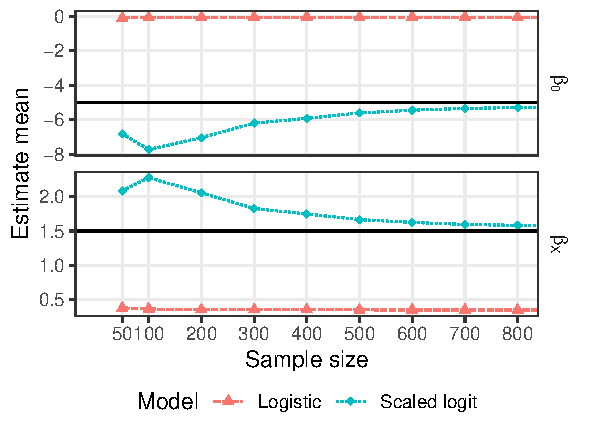
\includegraphics[width=0.69\textwidth]{../logistic-plot/vary_nsam_mean.pdf}
	\caption{
		Simulation results of fitting the standard logistic and the scaled logit models to the same simulated datasets. 10,000 datasets were simulated. Shown is the mean of the regression estimates from the standard logistic (the dashed line) and the scaled logit (the dotted line). Points indicate parameter values at which the simulations were performed. The solid lines are the true parameter values.
	}
	\label{SclrMean}
\end{figure}

When the unexposed subset of the population is present in the sample, the baseline risk $\lambda$ decreases. This does not necessarily bias the estimates of $\beta_0$ and $\beta_X$ but it can increase their standard errors.

To demostrate the effect of including the unexposed population into the analysis on the standard errors of the parameter estimates, we simulated 10,000 observations from the model

\[
	\begin{gathered}
		P(Y=1) = \frac{P(E=1)\text{exp}(\theta)}{(1+\text{exp}(\theta))(1+\text{exp}(\beta_0+\beta_X X))} \\
		\theta = \text{log}(\frac{\lambda}{1-\lambda}) \\
		\lambda = 0.5 \quad \beta_0 = -5 \quad \beta_T = 1.5 \\
		X \sim N(2, 2^2)
	\end{gathered}
\]

at the following values of \(P(E=1)\): 0.1, 0.2, 0.3, 0.4, 0.5, 0.6, 0.7, 0.8, 0.9, 1.

We then fit the scaled logit model using maximum likelihood to all data (general population, unexposed included) and the subset with just the exposed (unexposed excluded). The results of 10,000 simulations at each value of \(P(E=1)\) are in Figure \ref{fig:sclr-lowbase}.

\begin{figure}[htp]
	\centering
	\includegraphics[width=1\textwidth]{../sclr-lowbase/sim-plot/plot2.pdf}
	\caption{
		The results of 10,000 simulations at each parameter combination. Points represent values at which simulations were performed. Points and lines are colored based on the estimated term they belong to. The solid lines and triangles show estimated mean (left panel) and mean standard error (right panel) of estimates obtained from fitting models to the exposed population (i.e.,~unexposed excluded). The dashed lines and rhombi show the same for the general population (i.e.,~unexposed included).
	}
	\label{fig:sclr-lowbase}
\end{figure}

As expected, including the unexposed into the analysis has the effect of lowering the estimated baseline probability but has no appreciable effect on the expected estimates of the other parameters.

Including the unexposed into the anlalysis also has the effect of increasing the expected standard errors of the \(\beta_0\) and $\beta_X$ parameters (especially the intercept \(\beta_0\)) by 5-10\% when the exposed proportion is less then 50\%. As a result, it is advisable to limit the sample to those exposed, if possible.
